Battle Module
\begin{figure}[h]
\centering
\begin{center}
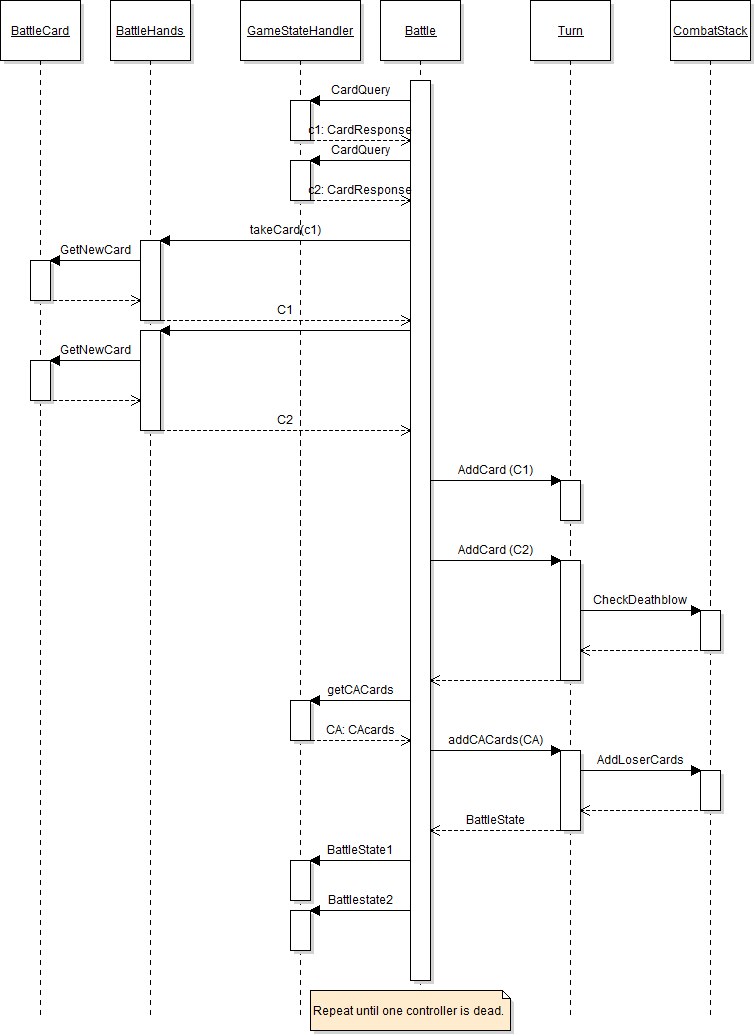
\includegraphics{diagrams/BattleSequenceDiagram.png}
\end{center}
\caption{A sequence diagram of one turn for each participant in a battle.}
\label{fig:battle_sequence_diagram}
\end{figure}

\begin{figure}[h]
\centering
\begin{center}
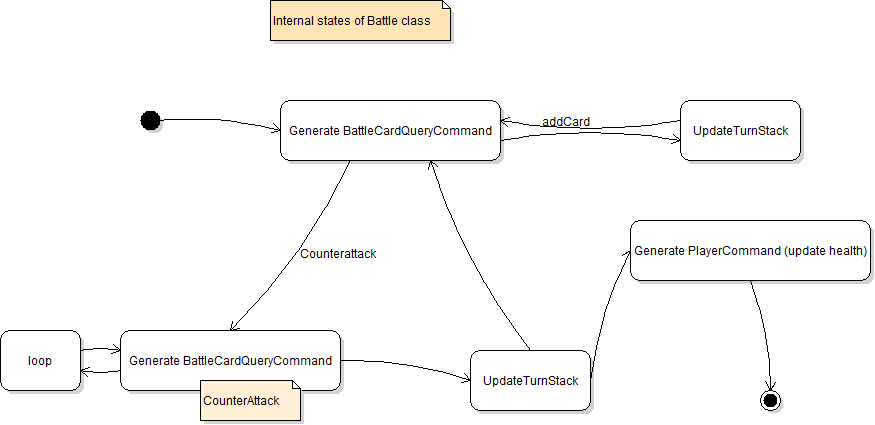
\includegraphics{diagrams/BattleStateDiagram.png}
\end{center}
\caption{A state diagram explaining the internal states of the Battle class.}
\label{fig:battle_state_diagram}
\end{figure}


A battle is conducted between two heroes controlled either by human players or by the AI. For more information on how a battle is conducted, see use case \ref{fightopponent}.

Diagram \ref{fig:battle_sequence_diagram} models one turn out of many in a battle. The \emph{GameStateHandler} communicates with human players and the AI through means not shown in this diagram, and the response is in the form of a card in the respective participant's battle hand. The class \emph{Battle} acts as a mediator between the heroes, their battle hands and \emph{turn}. A battle hand is composed of the five cards currently available to the respective player. The turn class contains the logic determining the winner of a single battle turn by comparing the chosen cards and possible lingering effects from previous rounds (specifically \emph{death blows}, see use case \ref{fight_deathblow}). When a turn ends, the losers' cards are added to the combat stack.

Diagram \ref{fig:battle_state_diagram} models the behaviour of the battle class from the start until the end of a battle.

\begin{figure}[h]
\centering
\begin{center}
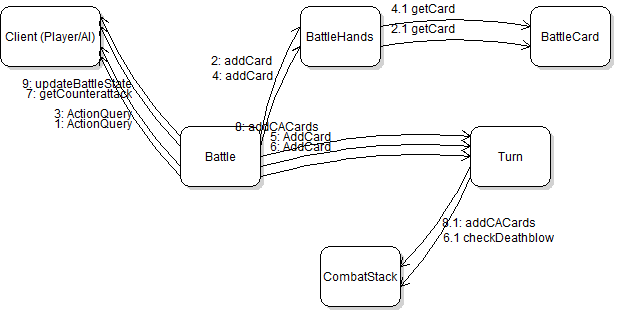
\includegraphics{diagrams/CounterAttackCommDiagram.png}
\end{center}
\caption{A diagram explaining the communication between the participating classes when a counter attack is possible.}
\label{fig:counter_attack_comm_diagram}
\end{figure}

A counter attack is possible in each turn for the losing participant given certain circumstances. For more detail on counter attack see use case \ref{fight_counterattack}. Diagram \ref{fig:counter_attack_comm_diagram} models the communication between the classes participating in a single turn when a counter attack is possible.


\begin{figure}[h]
\centering
\begin{center}
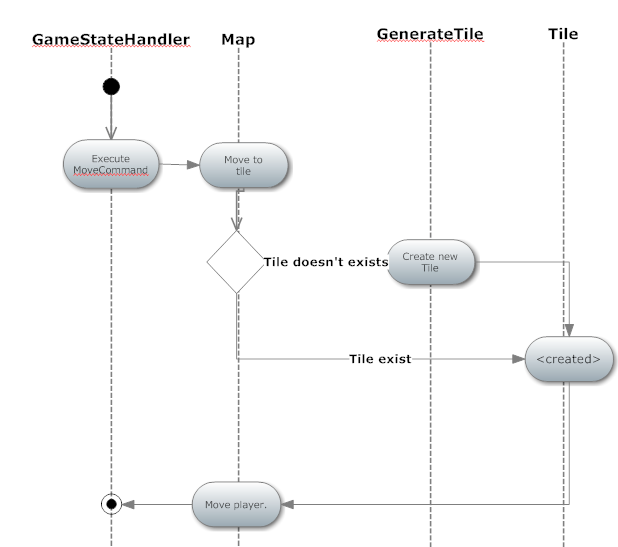
\includegraphics{diagrams/moveActivityDiagram.png}
\end{center}
\caption{An activity diagram explaining the process of a hero moving to a new square and the possible creation of a new tile.}
\label{fig:move_activity_diagram}
\end{figure}

Diagram \ref{fig:move_activity_diagram} models the process of a hero moving to a new room. For further information on how a move is carried out, see use case \ref{moveoutofroom}. A \emph{tile} is created if the room has previously not been visited, otherwise the hero simply moves to the new room.



